\section{Introduction}
\label{sec:intro}

Robots frequently need to change a scene before the intended operation becomes feasible. We study a class of \emph{bimanual exposure-and-execution} tasks in which one or both arms first manipulate a deformable occluder to reveal a target, subsequently operate on the target, and finally restore the surrounding scene. This structure appears in everyday activities, such as lifting a cloth to remove an object underneath and replacing the cloth, and in surgery, where tissue retraction establishes visibility and access for a subsequent intervention~\cite{attanasio2020retraction,pore2021retraction}. These tasks are sequential, but their difficulty is not merely the length of the action sequence: the outcome of each operation establishes, or destroys, the physical and perceptual conditions required by the next. Related dependencies arise in manipulation-based object search~\cite{dogar2014search,danielczuk2019mechanical} and preparatory manipulation~\cite{wan2020preparatory,shen2026bipremanip}. Figure~\ref{fig:taskoverview} shows the complete task considered here, from exposure through target manipulation to restoration.

\begin{figure}[t]
\centering
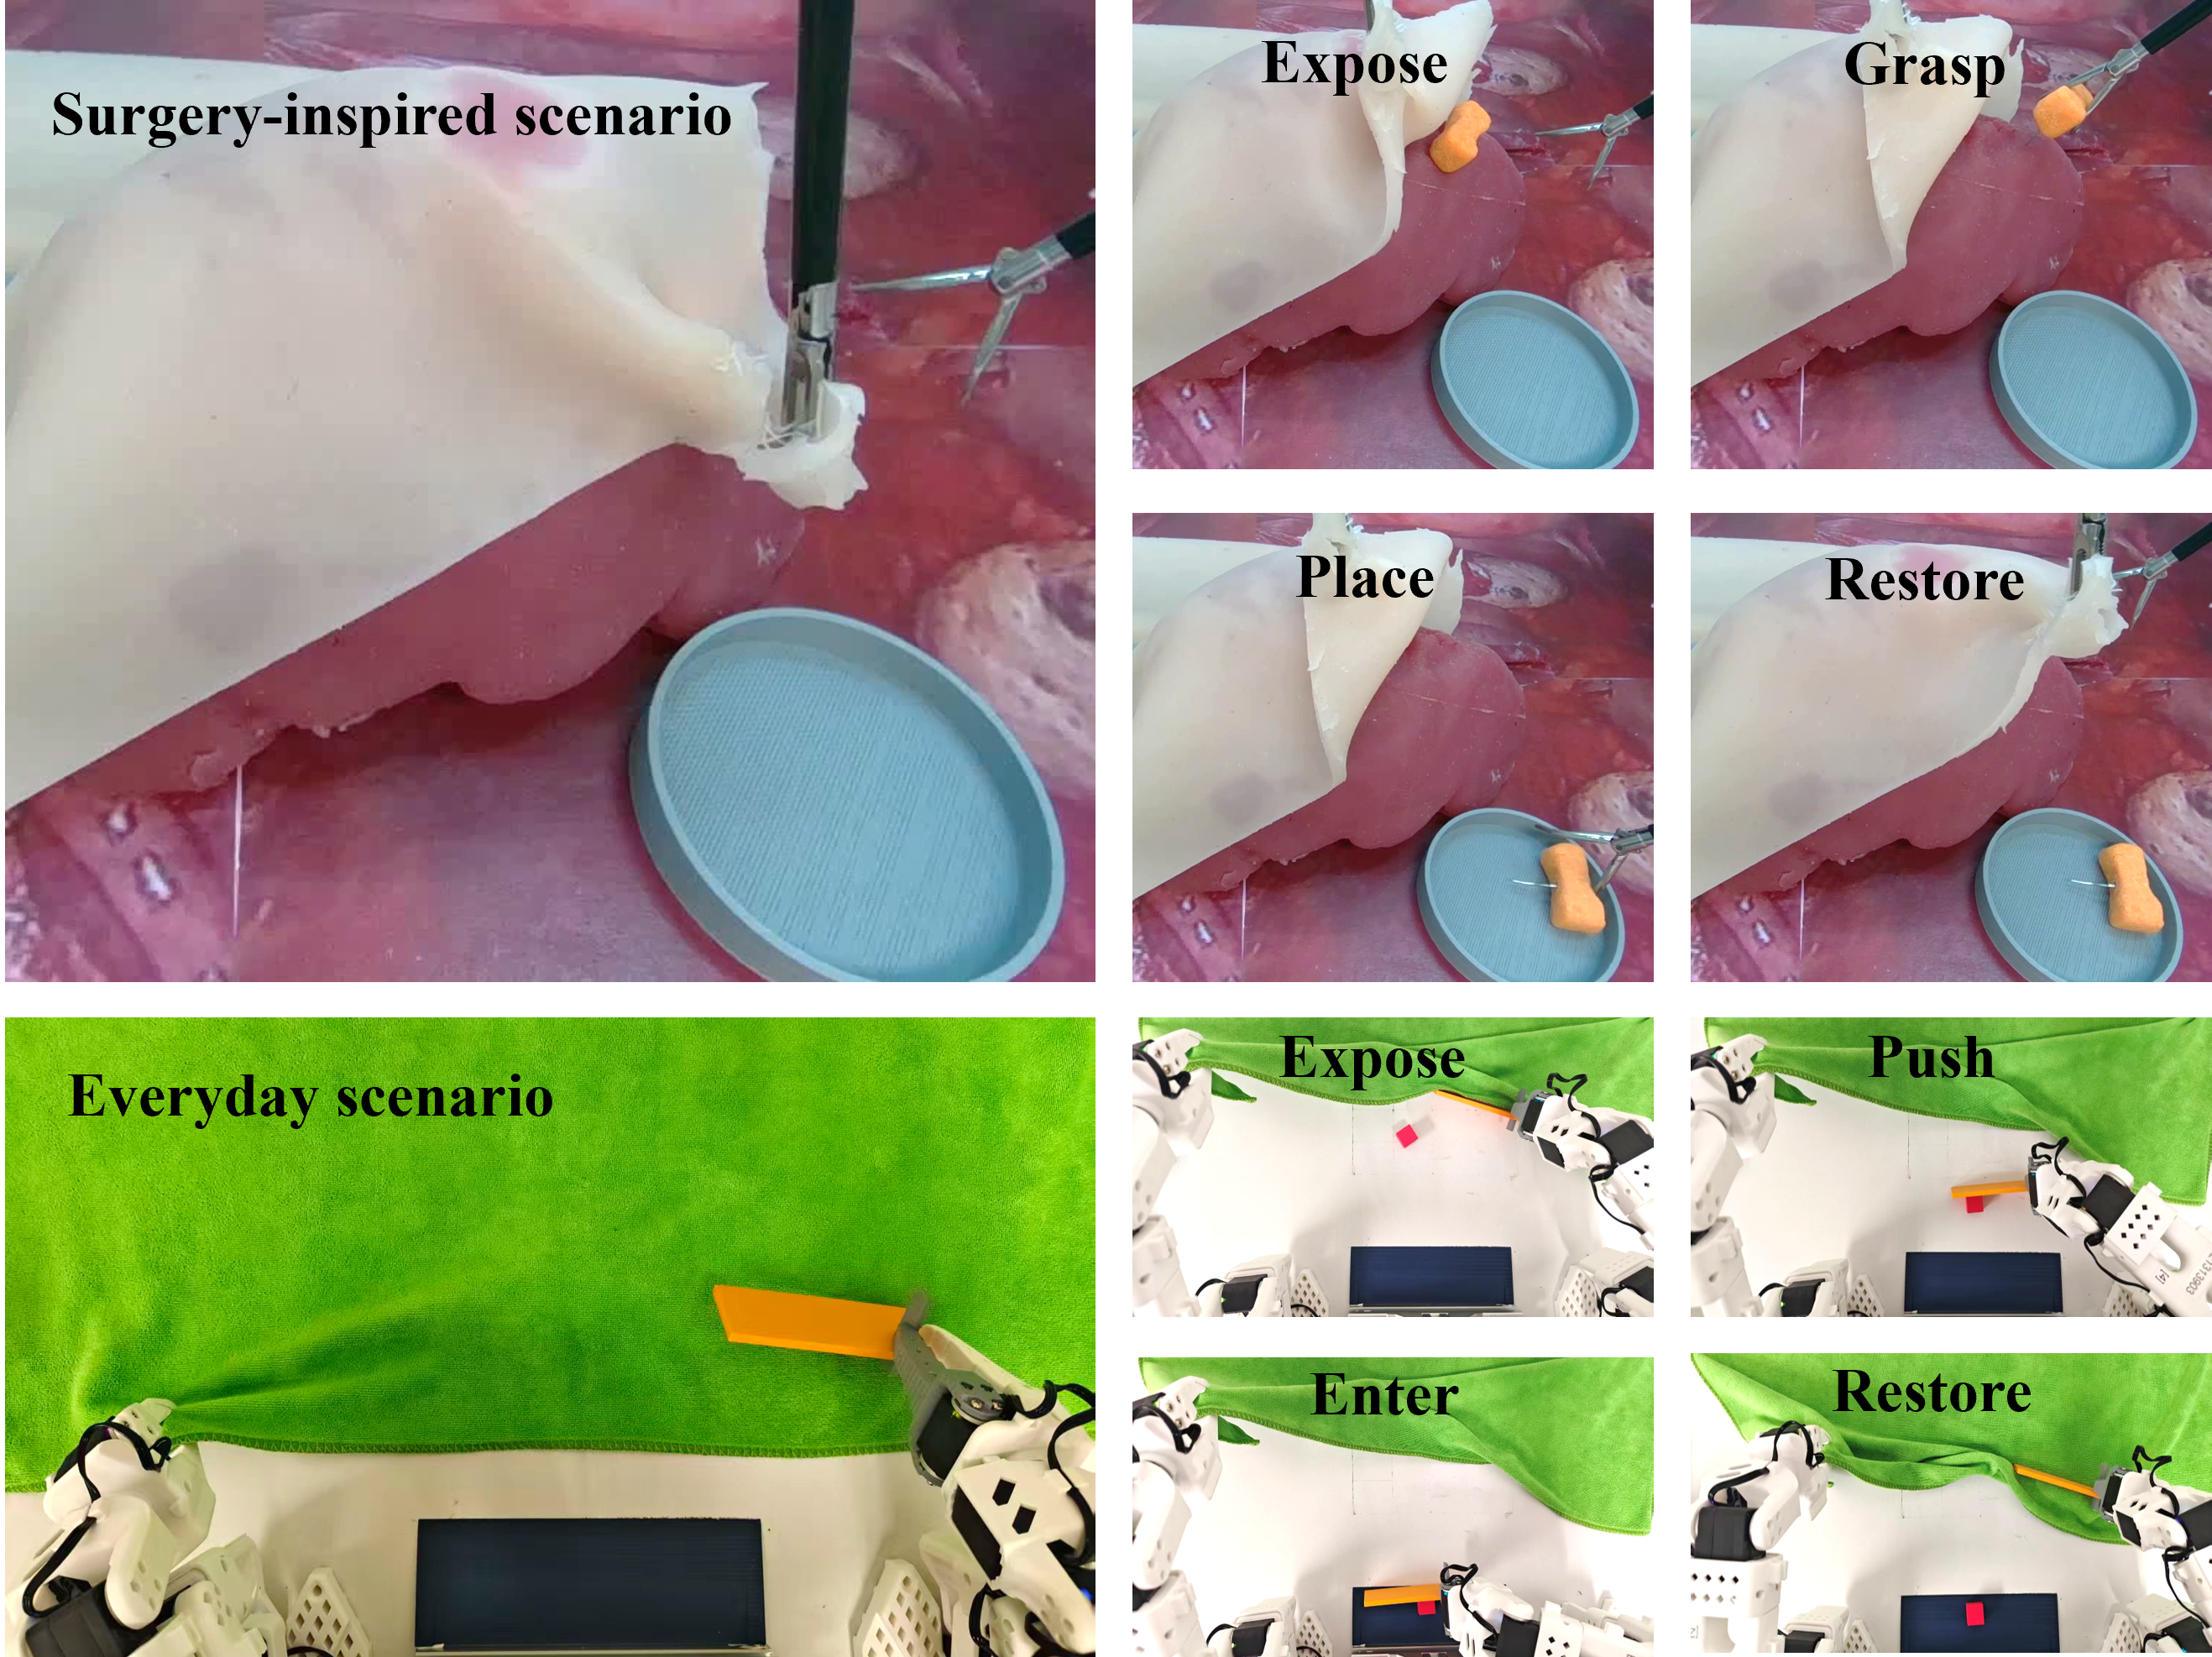
\includegraphics[width=\columnwidth]{myfigure/taskoverview1.png}
\caption{Overview of our bimanual exposure-and-execution tasks. The robot needs to expose an occluded target, manipulate it into a designated region, and restore the deformable covering by executing the sequences of operations displayed on the right.}
\label{fig:taskoverview}
\end{figure}

Exposure and execution couple perception, contact, and coordination in ways that make complete-task success substantially harder than performing the visible terminal operation alone. A deformable covering has a high-dimensional configuration and can fold, slip, or re-occlude the target after contact. The two arms take changing and often asymmetric roles: one arm may maintain or enlarge the exposed region while the other approaches the target, after which both must coordinate target transfer and restoration. Moreover, exposure is not a binary, isolated subgoal. An action can reveal part of the target yet leave insufficient tool clearance, displace the target, or place the occluder where it obstructs a later motion. The policy must therefore use visual feedback to track task conditions---including target visibility and the spatial relationships among the occluder, tools, target, and goal---and adapt later actions to the actual outcome of earlier interactions. Because complete success requires all of these conditions to remain compatible, a locally plausible action can still cause failure several operations later.

Visuomotor imitation learning is attractive for such contact-rich tasks because it can learn perception and control directly from demonstrations without an explicit model of deformable-object dynamics. Action Chunking with Transformers (ACT) learns temporally coherent bimanual commands~\cite{zhao2023act}, while Diffusion Policy represents multimodal action sequences through conditional denoising~\cite{chi2023diffusion}. These policy classes have enabled coordinated and multistage behaviors in systems such as Mobile ALOHA and UMI~\cite{fu2024mobilealoha,chi2024umi}. Explicit temporal abstractions provide another route: sequential manipulation can be represented with learned primitives or geometric constraints~\cite{liang2022sensorimotor,perez2017clearn}, and hierarchical policies can select, retry, and compose skills over long horizons~\cite{gupta2020relay,luo2024cable}. In this work, we ask a complementary question: when learning a single closed-loop action-chunk policy from a fixed and limited demonstration set, what information should its representation preserve so that subsequent actions remain compatible with the evolving task state?

Standard behavior cloning answers this question only indirectly through action-prediction loss. This is problematic for two related reasons. First, small errors can move the robot to histories that are weakly represented in the demonstrations, after which error compounds over the remaining horizon~\cite{ross2011,laskey2017dart}. Second, low demonstration loss does not by itself identify why the expert selected an action. A high-capacity policy may exploit visual or temporal correlations that predict demonstrated commands while omitting the physical relations that determine whether those commands remain appropriate; this issue is closely related to causal confusion and copycat behavior in imitation learning~\cite{dehaan2019,wen2020copycat}. Supplying object-centric features or semantic channels can reduce visual complexity, but their presence at the input does not guarantee that the internal representation used for action generation retains the particular visibility and geometric relations needed by the task. This distinction is especially consequential in exposure-and-execution tasks, where similar arm configurations can require different continuations depending on what the preceding interaction actually exposed or displaced.

We therefore use \emph{task-aware imitation learning} in a specific, operational sense: in addition to matching expert actions, the policy is trained so that selected task conditions remain recoverable from the representation that generates those actions. Our framework derives semantic masks for task entities and converts them into descriptors of target exposure and interaction geometry, including visible area, tool--target displacement, and target--goal distance. Learnable task queries integrate visual and proprioceptive observations; descriptor heads supervise the encoded query tokens, which are also available to the action decoder. This design differs from merely appending a segmentation image: semantic inputs provide object-level structure, whereas query supervision explicitly encourages the action-generating representation to preserve chosen task information. Because dense labels are costly, a quality-aware iterative annotation procedure expands three manually reviewed seed trajectories into semantic supervision over 102 additional trajectories, retains three disjoint trajectories for diagnostic monitoring, and uses temporal and structural tests to screen unreliable pseudo-labels.

The representation design is motivated by a task-level analysis rather than by the assumption that semantics automatically improve control. We first relate coordinated action error over the interaction horizon to complete exposure-and-execution failure. We then separate two requirements for transferring performance from demonstrations to deployment: coverage of deployment histories in the learned representation and preservation of information from which expert bimanual commands can be reconstructed. The resulting conditional bounds clarify both the intended benefit and the limitation of descriptor supervision: it targets a measurable representation error term, but successful execution still depends on coverage, action sensitivity, and whether the selected descriptors adequately explain expert choices.

We evaluate all policies using the same fixed set of 108 real-robot demonstrations. The test comprises 480 trials across five policies, four object types, and 12 initial positions. Our full method succeeds in 92 of 96 trials (95.8\%), compared with 54 of 96 (56.2\%) for ACT and 50 of 96 (52.1\%) for Diffusion Policy. In a $2\times2$ factorial ablation, semantic inputs alone reach 60 of 96 successes and supervised task queries alone reach 72 of 96; combining them yields the strongest complete-task performance. The improvement is achieved without additional policy interaction data and without introducing an explicit phase label or hierarchical skill selector.

The main contributions of this work are:
\begin{itemize}
    \item a formulation of bimanual exposure and execution that makes the dependence of later operations on achieved visibility and interaction geometry explicit, together with an analysis connecting action error and representation quality to complete-task failure;
    \item a task-aware visuomotor imitation framework that combines semantic observations with descriptor-supervised query tokens, directly encouraging task information to remain recoverable from the action-generating representation;
    \item a quality-aware iterative annotation procedure that expands sparse reviewed video masks into descriptor supervision while screening temporal and structural anomalies; and
    \item a controlled real-robot evaluation with 480 trials, including policy comparisons, factorial ablations, stage-wise outcomes, and a held-out object category, showing that semantic inputs and task-query supervision are complementary.
\end{itemize}
